\newpage
\def\thoigian{90}%--Thời gian
\de{Đề số 2}{Chương VII. Bất phương trình bậc hai một ẩn}



\begin{center}
	\textbf{PHẦN 1 - CÂU TRẮC NGHIỆM BỐN PHƯƠNG ÁN}
\end{center}
\Opensolutionfile{ans}[ans/ans-TN-ONTAPCHUONG7-DE2]

\begin{ex}%[0D7N1-1]%[Dự án D - đợt 3 NH24-25- Nguyễn Hoài Nam]
	Biểu thức nào dưới đây là tam thức bậc hai?
	\choice
	{\True $f(x)=3x^2+2x-5$ }
	{$f(x)=2x-4$ }
	{$f(x)=3x^3+2x-1$ }
	{$f(x)=x^4-x^2+1$ }
	\loigiai{Ta có $f(x)=3x^2+2x-5$ với $a=3\neq 0$ nên $f(x)$ tam thức bậc hai.}
\end{ex}
\begin{ex}%[0D7N1-1]%[Dự án D - đợt 3 NH24-25- Nguyễn Hoài Nam]
	Cho tam thức bậc hai $f(x)=ax^2+bx+c$, $(a\neq0)$ có bảng xét dấu như hình vẽ dưới đây
	\begin{center}
		
\begin{tikzpicture}
			\tkzTabInit[lgt=1.2,espcl=2.5]
			{$x$/0.6,$f(x)$/0.6}{$-\infty$,$x_1$,$x_2$,$+\infty$}
			\tkzTabLine{,-,$0$,+,$0$,-,}
		\end{tikzpicture}
	\end{center}
	Mệnh đề nào sau đây \textbf{sai}?
	\choice
	{\True Hệ số $a>0$}
	{$f(x)>0\Leftrightarrow x\in\left(x_1;x_2\right)$}
	{Tam thức có hai nghiệm}
	{$f(x)<0\Leftrightarrow x\in\left(-\infty;x_1\right)\cup\left(x_2;+\infty\right)$}
	\loigiai{
		Từ bảng xét dấu ta thấy tam thức có hai nghiệm phân biệt $x_1$; $x_2$.\\
		Và $f(x)>0\Leftrightarrow x\in\left(x_1;x_2\right)$; $f(x)<0\Leftrightarrow x\in\left(-\infty;x_1\right)\cup\left(x_2;+\infty\right)$.
	}
\end{ex}
\begin{ex}%[0D7N1-3]%[Dự án D - đợt 3 NH24-25- Nguyễn Hoài Nam]
	\immini
	{
		Cho hàm số bậc hai $y=f(x)$ có đồ thị như hình vẽ. Nhận định nào sau đây là đúng?
		\choice
		{\True $f(x)>0$ với $2<x<3$}
		{$f(x)<0$ với $x \leq 2$ hoặc $x \geq 3$}
		{$f(x)>0$ với $x<2$ hoặc $x>3$}
		{$f(x)<0$ với $2<x<3$}
	}
	{
		\begin{tikzpicture}[scale=.8,font=\footnotesize, line join=round, line cap=round, >=stealth]
			%%Nhập giới hạn đồ thị và hàm số cần vẽ
			\def \xmin{-1}
			\def \xmax{4}
			\def \ymin{-2}
			\def \ymax{1}
			\def \hamso{(2-\x)*(\x-3)}
			%\def \tiemcanxien{\x+1}
			%%Tự động
			\draw[->] (\xmin,0)--(\xmax,0) node[above] {$x$};
			\draw[->] (0,\ymin)--(0,\ymax) node[below left] {$y$};
			\draw (0,0) node [below right] {$O$};
			\draw (2,0)node[above]{$2$}
			(3,0)node[above]{$3$};
			\begin{scope}
				\clip (\xmin+0.01,\ymin+0.01) rectangle (\xmax-0.01,\ymax-0.01);
				\draw[samples=350,domain=\xmin+0.01:\xmax-0.01,smooth,variable=\x] plot (\x,{\hamso});
			\end{scope}
		\end{tikzpicture}
		
	}
	\loigiai{
		Từ đồ thị suy ra $f(x)>0$ với $2<x<3$.
	}
\end{ex}
\begin{ex}%[0D7H1-3]%[Dự án D - đợt 3 NH24-25- Nguyễn Hoài Nam]
	\immini
	{
		Dựa vào đồ thị hàm số bậc hai $f(x)=ax^2+bx+c$ (như hình bên), hãy chọn khẳng định đúng trong các khẳng định dưới đây.
		\choice
		{$f(x)\geq 0$ khi $x\in [-1;3]$}
		{Đồ thị hàm số luôn nằm trên trục hoành}
		{$f(x)<0$ khi $x\in (-\infty;-1)\cup (3;+\infty)$}
		{\True $f(x)\geq 0$ khi $x\in [3;+\infty)$}
	}
	{
		\begin{tikzpicture}[font=\footnotesize,line cap=round,line join=round,>=stealth, declare function={f(\x)=(\x)^2-2*(\x)-3;},scale=.7]
			\draw[->] (-2,0)--(4,0) node[shift={(-40:.2)}]{$x$};
			\draw[->] (0,-4)--(0,1) node[shift={(20:.2)}]{$y$};
			\draw[samples=100,smooth,domain=-1.23:3.23] plot (\x,{f(\x)});
			\fill (0,0) circle(1pt) node[shift={(-135:.3)}]{$O$} (-1,0) circle(1pt) node[shift={(-135:.35)}]{$-1$} (0,-3) circle(1pt) node[shift={(-165:.3)}]{$-3$} (3,0) circle(1pt) node[shift={(-45:.3)}]{$3$};
		\end{tikzpicture}
	}
	\loigiai
	{
		Đồ thị hàm số $f(x)=ax^2+bx+c$ cắt trục hoành tại hai điểm có hoành độ lần lượt là $-1$, $3$.\\
		Phần đồ thị của hàm số $f(x)=ax^2+bx+c$ không nằm phía dưới trục hoành ứng với $x\in (-\infty;-1]\cup [3;+\infty)$. Do đó, $f(x)\geq 0$ khi $x\in (-\infty;-1]\cup [3;+\infty)$.\\
		Phần đồ thị của hàm số $f(x)=ax^2+bx+c$ nằm phía dưới trục hoành ứng với $x\in (-1;3)$. Do đó, $f(x)< 0$ khi $x\in (-1;3)$.
	}
\end{ex}
\begin{ex}%[0D4B5-2]%[Dự án D - đợt 3 NH24-25- Nguyễn Hoài Nam]
	Bất phương trình $-x^2+2x+3<0$ có tập nghiệm là
	\choice
	{$\left(-1;3\right)$}
	{$\left(-3;1\right)$}
	{$\left[-1;3\right]$}
	{\True$\left(-\infty;-1 \right) \cup \left(3;+\infty\right)$}
	\loigiai{
		Ta có $-x^2+2x+3<0\Leftrightarrow \hoac{&x<-1\\&x>3.}$ \\
		Vậy tập nghiệm của bất phương trình là $S=\left(-\infty;-1\right)\cup\left(3;+\infty\right)$.
	}
\end{ex}

\begin{ex}%[0D7N2-2]%[Dự án D - đợt 3 NH24-25- Nguyễn Hoài Nam]
	Tìm tất cả giá trị của $x$ để $-x^2-4x+5\ge 0$.
	\choice
	{$x\in \left(-\infty;-1\right]\cup \left[5;+\infty \right)$}
	{$x\in \left[-1; 5\right]$}
	{\True $x\in \left[-5; 1\right]$}
	{$x\in \left(-5; 1\right)$}
	\loigiai{
		Xét tam thức $f(x)=-x^2-4x+5$. Ta có
		\begin{itemize}
			\item $a=-1< 0$;
			\item $\Delta=36> 0$ nên  tam thức $f(x)$ có hai nghiệm $x=1$ và $x=-5$.
		\end{itemize}
		Bảng xét dấu
		\begin{center}
			
\begin{tikzpicture}[>=stealth]
				\tkzTabInit[nocadre=false,lgt=1.5,espcl=2,deltacl=0.6]{$x$/.7 ,$f(x)$/.7}
				{$-\infty$ , $-5$ , $1$ , $+\infty$}
				\tkzTabLine{ , - , $0$ , + , $0$ , - , }
			\end{tikzpicture}
		\end{center}
		Suy ra $f(x)\ge 0$ khi $-5\le x\le 1$.
	}
\end{ex}

\begin{ex}%[0D7H2-2]%[Dự án D - đợt 3 NH24-25- Nguyễn Hoài Nam]
	Tập nghiệm của bất phương trình $x^2-2x<0$ là
	\choice
	{\True $S = \left(0;2\right)$}
	{$S= \mathbb{R}$}
	{$S= (-\infty;0)\cup (2;+\infty)$}
	{$S= \left(1;+\infty \right)$}
	\loigiai{ Xét $f(x)=x^2-2x$.\\
		$f(x)=0\Leftrightarrow \hoac{&{x=0} \\
			&{x=2}
			&}$ và $a=1> 0$.\\
		Bảng xét dấu
		\begin{center}
			
\begin{tikzpicture}[>=stealth]
				\tkzTabInit[nocadre=false,lgt=1.5,espcl=2,deltacl=0.6]{$x$/.7 ,$f(x)$/.7}
				{$-\infty$ , $0$ , $2$ , $+\infty$}
				\tkzTabLine{ , + , $0$ , - , $0$ , + , }
			\end{tikzpicture}
		\end{center}
		Do đó $f(x) < 0,\forall x\in \left(0;2\right)$.\\
		Vậy tập nghiệm của bất phương trình là $S = \left(0;2\right)$.
	}
\end{ex}

\begin{ex}%[0D7H2-2]%[Dự án D - đợt 3 NH24-25- Nguyễn Hoài Nam]
	Tam thức bậc hai $f(x)=-x^2+3x-2$ nhận giá trị không âm khi và chỉ khi
	\choice
	{$x\in \left(-\infty;1\right]\cup \left[2;+\infty \right)$}
	{\True $x\in \left[1;2\right]$}
	{$x\in \left(1;2\right)$}
	{$x\in \left(-\infty;1\right)\cup \left(2;+\infty \right)$}
	\loigiai{
		Ta có
		\[f(x)=0\Leftrightarrow-x^2+3x-2=0\Leftrightarrow \hoac{&{x=1} \\
			&{x=2.}
			&}
		\]
		Bảng xét dấu $f(x)$
		\begin{center}
			
\begin{tikzpicture}[>=stealth]
				\tkzTabInit[nocadre=false,lgt=1.5,espcl=2,deltacl=0.6]{$x$/.7 ,$f(x)$/.7}
				{$-\infty$ , $1$ , $2$ , $+\infty$}
				\tkzTabLine{ , - , $0$ , + , $0$ , - , }
			\end{tikzpicture}
		\end{center}	
		Tam thức bậc hai $f(x)=-x^2+3x-2$ nhận giá trị không âm khi và chỉ khi $f(x)\ge 0\Leftrightarrow x\in \left[1;2\right]$.
	}
\end{ex}

\begin{ex}%[0D7H3-1]%[Dự án D - đợt 3 NH24-25- Nguyễn Hoài Nam]
	Tổng tất cả các nghiệm của phương trình $\sqrt{x^2 + 2x - 3} = \sqrt{15-5x}$ là
	\choice
	{$7$}
	{\True $-7$}
	{$6$}
	{$4$}
	\loigiai{
		Bình phương hai vế của phương trình ta được 
		\[
		x^2 + 2x -3 = 15-5x \Rightarrow x^2  + 7x-18 = 0\Rightarrow \hoac{&x=2\\ &x=-9.}
		\]	
		Thử lại ta thấy $x=2$ và $x=-9$ đều thoả mãn nên tổng các nghiệm của phương trình là 
		\[
		2+(-9)= -7.
		\]
	}
\end{ex}

\begin{ex}%[0D7H3-2]%[Dự án D - đợt 3 NH24-25- Nguyễn Hoài Nam]
	Số nghiệm nguyên của phương trình $\sqrt{x^2 +10x-5} = 2(x-1)$ là
	\choice
	{\True $0$}
	{$2$}
	{$3$}
	{$1$}
	\loigiai{
		Ta có phương trình tương đương với
		\[
		\heva{&2(x-1)\ge 0\\ &x^2+10x-5 = [2(x-1)]^2}
		\Leftrightarrow \heva{&x\ge 1\\ &3x^2 - 18x  +9 = 0}
		\Leftrightarrow \heva{&x\ge 1\\ &x=3\pm 6}
		\Leftrightarrow x=3+\sqrt{6}.
		\]	
		Vậy phương trình không có nghiệm nguyên.
	}
\end{ex}
\begin{ex}%[0D7H3-1]%[Dự án D - đợt 3 NH24-25- Nguyễn Hoài Nam]
	Số nghiệm của phương trình $\sqrt{2x-1}+2=x$ là
	\choice
	{\True $1$}
	{$2$}
	{$0$}
	{$4$}
	\loigiai{
		Ta có $\sqrt{2x-1}+2=x \Rightarrow \sqrt{2x-1}=x-2$.\\
		Bình phương hai vế của phương trình, ta được 
		$$2x-1=x^2-4x+4 \Rightarrow x^2-6x+5=0 \Rightarrow \hoac{&x=1\,\text{ (loại)}\\&x=5\,\text{ (nhận).}}$$
		Vậy phương trình có $1$ nghiệm.
	}
\end{ex}
\begin{ex}%[0D7H3-1]%[Dự án D - đợt 3 NH24-25- Nguyễn Hoài Nam]
	Một nghiệm của phương trình $\sqrt{3x^2+6x+3}=\sqrt{2x^2-5x+3}$ là
	\choice
	{\True $x=-11$}
	{$x=1$}
	{$x=11$}
	{$x=4$}
	\loigiai{
		Bình phương hai vế của phương trình ta được
		\begin{eqnarray*}
			& & 3x^2+6x+3=2x^2-5x+3\\
			&\Leftrightarrow & x^2+11x=0\\
			& \Leftrightarrow & \hoac{&x=0\\&x=-11.}
		\end{eqnarray*}
		Thử lại, ta có nghiệm của phương trình là $x=0$ và $x=-11$.
	}
\end{ex}



\Closesolutionfile{ans}
%\begin{center}
%	\textbf{ĐÁP ÁN}
%	\inputansbox{10}{ans/ans}	
%\end{center}


\begin{center}
	\textbf{PHẦN 2 - CÂU TRẮC NGHIỆM ĐÚNG SAI}
\end{center}

\Opensolutionfile{ans}[ans/answer-DS-ONTAPCHUONG7-DE2]
\begin{ex}%[0D7V3-5]%[Dự án D - đợt 3 NH24-25- Nguyễn Hoài Nam]
	Cho đồ thị của hàm số bậc hai $y = f(x)$ như sau
	\begin{center}
		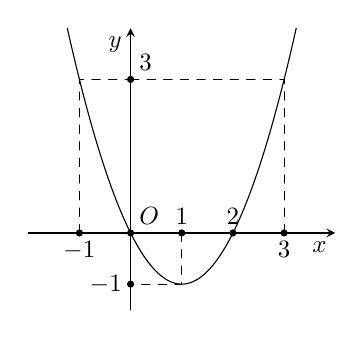
\begin{tikzpicture}[line join=round, line cap=round,>=stealth,scale=.65]
			\tikzset{every node/.style={scale=0.9}}
			\def\xmin{-2} \def\xmax{4}\def\ymin{-1.5}\def\ymax{4}
			\draw[->] (\xmin,0)--(\xmax,0) node[below left] {$x$};
			\draw[->] (0,\ymin)--(0,\ymax)  node[below left] {$y$};
			\clip (\xmin,\ymin) rectangle (\xmax,\ymax);
			\draw[dashed] (-1,0)|-(0,3) (1,0)|-(0,-1) (3,0)|-(0,3);
			\fill (0,0)node[above right]{$O$} circle(2pt)
			(3,0)node[below]{$3$} circle(2pt)
			(-1,0)node[below]{$-1$} circle(2pt)
			(0,3)node[above right]{$3$} circle(2pt)
			(1,0)node[above]{$1$} circle(2pt)
			(2,0)node[above]{$2$} circle(2pt)
			(0,-1)node[left]{$-1$} circle(2pt)
			;
			\begin{scope}
				\clip (\xmin,\ymin) rectangle (\xmax,\ymax);
				\draw[samples=200,domain=\xmin:\xmax,smooth,variable=\x] plot
				(\x,{(\x)^2-2*(\x)});
			\end{scope}
		\end{tikzpicture}
	\end{center}
	\choiceTF
	{\True Khi $x>2$ thì $f(x)>0$}
	{Bất phương trình $f(x)\le 0$ có tập nghiệm là đoạn $[-1;0]$}
	{\True Bất phương trình $f(x)\ge 3$ có $5$ nghiệm nguyên}
	{Phương trình $f^2(x) - 9 = 0$ có $4$ nghiệm}
	\loigiai{
		\begin{itemchoice}
			\itemch Dựa theo đồ thị hàm số $y=f(x)$, $f(x)>0$ khi và chỉ khi $x<0$ hoặc $x>2$. Nên khi $x>2$ thì $f(x)>0$.
			\itemch Dựa theo đồ thị hàm số $y=f(x)$, $f(x)\le 0$ khi và chỉ khi $0 \le x \le 2$. Vậy tập nghiệm $f(x)\le 0$ là đoạn $[0;2]$.
			\itemch Dựa theo đồ thị hàm số $y=f(x)$, $f(x)\le 3$ khi và chỉ khi $-1 \le x \le 3$. Vậy tập các nghiệm nguyên của bất phương trình $f(x)\le 3$ là $\{-1;0;1;2;3\}$. 
			\itemch Phương trình $f^2(x) - 9 = 0$ tương đương 
			$$f^2(x) = 9 \Leftrightarrow \hoac{&f(x)=3 \\ &f(x)=-3.}$$
			Dựa theo đồ thị hàm số $y=f(x)$ thì 
			\begin{itemize}
				\item Phương trình $f(x)=3$ có nghiệm $x=-1$ và $x=3$.
				\item Phương trình $f(x)=-3$ vô nghiệm (do tam thức bậc hai $f(x)$ có giá trị nhỏ nhất là $-1$).
			\end{itemize}
			Vậy phương trình $f^2(x)=9$ có $2$ nghiệm.
		\end{itemchoice}
	}
\end{ex}
\begin{ex}%[0D7H3-2]%[Dự án D - đợt 3 NH24-25- Nguyễn Hoài Nam]
	Cho biểu thức $f(x)=x^2-3x+2$
	\choiceTF
	{\True Biểu thức $f(x)=x^2-3x+2$ là một tam thức bậc hai}
	{\True $x=3$ là một nghiệm của bất phương trình $x^2-3x+2 \geq 0$}
	{Có 2 giá trị nguyên của $x$ để tam thức bậc hai $f(x)=x^2-3x+2<0$}
	{ Phương trình $\sqrt{f(x)}=2x-2$ có hai nghiệm phân biệt}
	\loigiai{
		\begin{itemchoice}
			\itemch Ta có biểu thức $f(x)=x^2-3x+2$ là một tam thức bậc hai.
			\itemch Vì $3^2-3\cdot3+2=2>0$ nên $x=3$ là một nghiệm của bất phương trình $x^2-3x+2 \geq 0$.
			\itemch Tam thức bậc hai $f(x)=x^2-3x+2$ có $\Delta=1>0$, hai nghiệm phân biệt là $x_1=1$, $x_2=2$ và $a=1>0$.\\
			Ta có bảng xét dấu $f(x)$ như sau
			\begin{center}
				
\begin{tikzpicture}[scale=1, font=\footnotesize, line join=round, line cap=round, >=stealth]
					\tkzTabInit[nocadre=false,lgt=1.2,espcl=2.5,deltacl=0.6]
					{$x$/0.6,$f(x)$/0.6}
					{$-\infty$,$1$,$2$,$+\infty$}
					\tkzTabLine{,+,0,-,0,+,}
				\end{tikzpicture}
			\end{center}
			Suy ra $f(x)=x^2-3x+2<0$ khi $x\in(1;2)$.\\
			Vậy không có giá trị nguyên của $x$ thỏa mãn.
			\itemch 
			\begin{eqnarray*}
				& & \sqrt{f(x)}=2x-2\\
				& \Leftrightarrow& \sqrt{x^2-3x+2}=2x-2\\
				& \Rightarrow & x^2-3x+2=(2x-2)^2\\
				&\Leftrightarrow & -3x^2+5x-2=0\\
				& \Leftrightarrow & \hoac{& x=1\\& x=\dfrac{2}{3}. }			
			\end{eqnarray*}
			Thử lại, nhận $x=1$, loại $x=\dfrac{2}{3}$.\\
			Vậy $\sqrt{f(x)}=2x-2$ có một nghiệm.
		\end{itemchoice}
	}
\end{ex}
\Closesolutionfile{ans}
%\inputansbox[2]{2}{ans/answer.tex}



\begin{center}
	\textbf{PHẦN 3 - CÂU TRẮC NGHIỆM TRẢ LỜI NGẮN}
\end{center}
\setcounter{ex}{0}
\Opensolutionfile{ans}[ans-KQ-ONTAPCHUONG7-DE2]


\begin{ex}%[0D7H3-1]%[Dự án D - đợt 3 NH24-25- Nguyễn Hoài Nam]
	Tổng các nghiệm của phương trình $\sqrt{x^2+2x-3}=\sqrt{15-5x}$ bằng bao nhiêu?
	\shortans{$-7$}
	\loigiai{
		\allowdisplaybreaks
		\begin{eqnarray*}
			\sqrt{x^2+2x-3}=\sqrt{15-5x}&\Leftrightarrow&\heva{
				& 15-5x\ge 0\\&{x^2}+2x-3=15-5x}\\ 
			&\Leftrightarrow&\heva{
				& x\le 3\\&{x^2}+7x-18=0}\\&\Leftrightarrow&\heva{
				& x\le 3\\&\hoac{& x=2\\& x=-9}}\\ 
			&\Leftrightarrow& \hoac{& x=2\\& x=-9.}
		\end{eqnarray*}
		Vậy $ S=2-9=-7$.}
\end{ex}
\begin{ex}%[0D7V2-7]%[Dự án D - đợt 3 NH24-25- Nguyễn Hoài Nam]
	Xét hệ toạ độ $Oth$ trên mặt phẳng, trong đó trục $Ot$ biểu thị thời gian $t$ (tính bằng giây) và trục $Oh$ biểu thị độ cao $h$ (tính bằng mét). Một quả bóng được đá lên từ điểm $A(0; 0{,}2)$ và chuyển động theo quỹ đạo là một cung parabol. Quả bóng đạt độ cao $8{,}5$ m sau 1 giây và đạt độ cao $6$ m sau 2 giây. Trong khoảng thời gian $(a;b)$ thì quả bóng vẫn chưa chạm đất. Tìm $b$ (kết quả làm tròn đến hàng phần trăm).
	\shortans{$2{,}55$}
	\loigiai{ 
		\begin{itemize}
			\item Giả sử hàm số có dạng $h=a t^2+bt+c$, trong đó $h$ là độ cao, $t$ là thời gian, $a, b, c$ là các hằng số cần tìm với $a\neq 0$.\\
			Quỹ đạo của quả bóng là một parabol đi qua điểm $A(0; 0{,}2)$ nên thay $t=0$ và $h=0{,}2$ vào hàm số ta được $c=0{,}2$.\\
			Suy ra $h=at^2+bt+0{,}2$.\\
			Lại có quả bóng đạt độ cao $8{,}5$ m sau $1$ giây và $6$ m sau $2$ giây, do đó quỹ đạo của bóng là parabol đi qua các điểm có tọa độ $(1; 8{,}5)$ và $(2; 6)$.\\
			Ta có hệ $\heva{&a+b+0{,}2=8{,}5\\
				&4a+2b+0{,}2=6\\}\Leftrightarrow \heva{&a=-5{,}4\\&b=13{,}7.\\}$\\
			Vậy hàm số bậc hai biểu thị quỹ đạo chuyển động của quả bóng là $h=-5{,}4t^2+13{,}7t+0{,}2$.
			\item Bóng chạm đất nếu khi độ cao $h=0$, vậy bóng chưa chạm đất khi độ cao $h>0$.\\
			Suy ra $- 5{,}4t^2+13{,}7t+0{,}2>0$, đây là bất phương trình bậc hai một ẩn với ẩn $t$.\\
			Tam thức bậc hai $-5{,}4t^2+13{,}7t+0{,}2$ có hai nghiệm $t_1=\dfrac{137}{108}-\dfrac{\sqrt{19\,201}}{108}$, $t_2=\dfrac{137}{108}+\dfrac{\sqrt{19\,201}}{108}$.\\
			Sử dụng định lí về dấu của tam thức bậc hai ta có \allowdisplaybreaks
			\begin{eqnarray*}
				&&-5{,}4 t^2+13{,}7t+0{,}2>0\\
				&\Leftrightarrow&\dfrac{137}{108}-\dfrac{\sqrt{19\,201}}{108}<t<\dfrac{137}{108}+\dfrac{\sqrt{19\,201}}{108}.
			\end{eqnarray*}
			Lại có thời gian $t>0$.\\
			Do đó $0<t<\dfrac{137}{108}+\dfrac{\sqrt{19\,201}}{108}$.\\
			Mà $\dfrac{137}{108}+\dfrac{\sqrt{19\,201}}{108}\approx 2{,}55$.\\
			Vậy trong khoảng thời gian từ $0$ đến $2{,}55$ giây thì bóng vẫn chưa chạm đất.
		\end{itemize}
	}
\end{ex}

\begin{ex}%[0D7V1-2]%[Dự án D - đợt 3 NH24-25- Nguyễn Hoài Nam]
	Tính tổng các giá trị nguyên của tham số $m$ để bất phương trình $x^2+2(m-2)x+2m-1\ge 0$ nghiệm đúng với mọi $x\in\mathbb{R}$.
	\shortans{$15$}
	\loigiai{
		Vì hệ số $a=1>0$, nên bất phương trình đã cho nghiệm đúng với mọi $x\in\mathbb{R}$ khi và chỉ khi
		$$\Delta =(m-2)^2-(2m-1)\le 0\Leftrightarrow  m^2-6m+5\le 0\Leftrightarrow  1\le m\le 5.$$
		Vậy tổng các giá trị nguyên của tham số $m$ là $1+2+3+4+5=15$.
	}
\end{ex}
\begin{ex}%[0D7V3-6]%[Dự án D - đợt 3 NH24-25- Nguyễn Hoài Nam]
	\immini{Để leo lên một bức tường, bác Nam dùng một chiếc thang có chiều dài cao hơn bức tường đó $1$ m. Ban đầu, bác Nam đặt chiếc thang mà đầu trên của chiếc thang đó vừa chạm đúng vào mép trên bức tường (tham khảo Hình a). Sau đó, bác Nam dịch chuyển chân thang vào gần chân tường thêm $0{,}5$ m thì bác Nam nhận thấy thang tạo với mặt đất một góc $60^{\circ}$ (tham khảo Hình b). Bức tường cao bao nhiêu mét (làm tròn kết quả đến hàng phần mười)?}
	{\begin{tikzpicture}[scale=0.8, font=\footnotesize,line join=round, line cap=round, >=stealth];
			\path
			(0,0) coordinate (O) node[below] {$C$}
			(2,5) coordinate (A)
			(0,5) coordinate (B)node[above] {$A$}
			(0.2,5.5) coordinate (B')
			(-2.5,0) coordinate (C)node[below] {$B$}
			(-1.8,0) coordinate (C')
			;
			\draw[very thick,color=orange,pattern=bricks] (O) rectangle (A);
			\draw[line width=4,blue] (B)--(C);
			\draw (O)--(C);
			\draw pic[draw,angle radius=2mm] {right angle = B--O--C'};
			\path (current bounding box.south) node[below] {Hình a)};
		\end{tikzpicture}
		\hfil
		\begin{tikzpicture}[scale=0.8, font=\footnotesize,line join=round, line cap=round, >=stealth];
			\path
			(0,0) coordinate (O) node[below] {$G$}
			(2,5) coordinate (A)
			(0,5) coordinate (B)node[left] {$D$}
			(0.2,5.5) coordinate (B')
			(-2.5,0) coordinate (C)
			(-1.8,0) coordinate (C')node[below] {$E$}
			;
			\draw[very thick,color=orange,pattern=bricks] (O) rectangle (A);
			\draw[line width=4,blue] (B')--(C');
			\draw (O)--(C);
			%\node[rectangle,name=node1,align=none,left] at ($ (C)!0.5!(B) $){$4$m};
			\pic["$60^\circ$"{shift={(1pt,0pt)}},draw,angle radius=4mm,angle eccentricity=1.79] {angle =O--C'--B'};
			\draw pic[draw,angle radius=2mm] {right angle = B'--O--C'};
			\path (current bounding box.south) node[below] {Hình b)};
		\end{tikzpicture}
	}
	\shortans{$4{,}7$}
	\loigiai{
		Gọi $x$ là chiều cao của bức tường. Điều kiện $x>0$, đơn vị: mét. \\
		Suy ra chiều dài của thang là $x+1$ m. \\
		Áp dụng định lí Py-ta-go trong hình 33a, ta được
		$$BC^2=(x+1)^2-x^2=2x+1 \Rightarrow BC=\sqrt{2x+1} \mathrm{~m}.$$
		Áp dụng hệ thức lượng trong tam giác vuông ở hình b, ta được
		$$
		\begin{aligned}
			DG=EG\cdot \tan 60^\circ &\Leftrightarrow x=\sqrt{3}\left(\sqrt{2x+1}-0{,}5\right) \\
			&\Leftrightarrow \sqrt{2x+1}=\dfrac{x}{\sqrt{3}}+0{,}5 
			\Leftrightarrow 2x+1=\left(\dfrac{x}{\sqrt{3}}+0{,}5\right)^2 \\
			&\Leftrightarrow \dfrac{x^2}{3}+\left(\dfrac{1}{\sqrt{3}}-2\right)x-\dfrac{3}{4}=0.
		\end{aligned}$$
		Giải phương trình trên (kết hợp điều kiện $x>0$) ta được $x\approx 4{,}7$.
	}
\end{ex}





\Closesolutionfile{ans}



\begin{center}
	\textbf{PHẦN 4 - TỰ LUẬN}
\end{center}


\begin{ex}%[0D7H2-3]%[Dự án D - đợt 3 NH24-25- Nguyễn Hoài Nam]
	Giải bất phương trình $\left(x^2-3x+2\right)\left(x^2-1\right)\le 0$.
	\loigiai{
		Bất phương trình tương đương với
		\begin{eqnarray*}
			&& (x-1)(x-2)(x-1)(x+1)\le 0\\
			& \Leftrightarrow & (x-1)^2(x-2)(x+1)\le 0\\
			& \Leftrightarrow & \hoac{& (x-1)^2=0 \\ & (x-2)(x+1)\le 0}\quad (\text{vì}\ (x-1)^2\ge 0.)\\
			& \Leftrightarrow & \hoac{& x=1 \\ & -1\le x\le 2}\\
			& \Leftrightarrow & -1\le x\le 2.
		\end{eqnarray*}
		Vậy tập nghiệm của bất phương trình là $[-1;2]$.
	}
\end{ex}
\begin{ex}%[0D7V2-7]%[Dự án D - đợt 3 NH24-25- Nguyễn Hoài Nam]
	Một công ty du lịch thông báo giá tiền cho chuyến đi tham quan của một nhóm khách du lịch như sau: $50$ khách đầu tiên có giá là $300\,000$ đồng/người. Nếu có nhiều hơn $50$ người đăng kí thì cứ có thêm $1$ người, giá vé sẽ giảm $5\,000$ đồng/người cho toàn bộ hành khách.
	\begin{enumerate}[a)]
		\item Gọi $x$ là số lượng khách từ người thứ $51$ trở lên của nhóm. Biểu thị doanh thu theo $x$.
		\item Số người của nhóm khách du lịch nhiều nhất là bao nhiêu thì công ty không bị lỗ? Biết rằng chi phí thực sự cho chuyến đi là $15\,080\,000$ đồng.
	\end{enumerate}
	\loigiai{
		\begin{enumerate}[a)]
			\item Do $x$ là số lượng khách thứ $51$ trở lên nên $x>0$.\\
			Cứ thêm $1$ người thì giá còn $(300\,000-5 \,000\cdot1)$ đồng/người cho toàn bộ hành khách.
			Thêm $x$ người thì giá còn $(300 \,000-5 \,000\cdot x)$ đồng/người cho toàn bộ hành khách.\\
			Doanh thu theo $x$ là $(50+x)\cdot(300\,000-5\,000\cdot x)$ đồng.
			\item Do chi phí thực sự cho chuyến đi là $15\,080\,000$ đồng nên để công ty không bị lỗ thì doanh thu phải lớn hơn hoặc bằng $15\,080\,000$ đồng
			Khi đó:
			$$
			\begin{aligned}
				&(50+x) \cdot(300\,000-5\,000 x) \geq 15\,080\,000 \\
				&\Leftrightarrow(50+x) \cdot 5\,000 \cdot(60-x) \geq 15\,080\,000 \\
				&\Leftrightarrow(x+50)(60-x) \geq 3\,016 \\
				&\Leftrightarrow-x^{2}+10 x+3000 \geq 3\,016 \\
				&\Leftrightarrow-x^{2}+10 x-16 \geq 0 \\
				&\Leftrightarrow 2 \leq x \leq 8
			\end{aligned}
			$$
			Vậy số người của nhóm du khách nhiều nhất là $58$ người thì công ty không bị lỗ.
		\end{enumerate}
	}
\end{ex}
\begin{ex}[Trích đề thi TN THPT 2025]%[0D7V2-7]%[Dự án D - đợt 3 NH24-25- Nguyễn Hoài Nam]
	Nếu một doanh nghiệp sản xuất $x$ sản phẩm trong một tháng ($x \in \mathbb{N}^*$; $1 \leq x \leq 4\,500$) thì doanh thu nhận được khi bán hết số sản phẩm đó là $F(x)= -0{,}01x^2 + 300x$ (nghìn đồng), trong khi chi phí sản xuất bình quân cho mỗi sản phẩm là $G(x)=\dfrac{30\,000}{x} + 200$ (nghìn đồng). Giả sử số sản phẩm sản xuất ra luôn được bán hết. Trong một tháng, doanh nghiệp đó cần sản xuất ít nhất bao nhiêu sản phẩm để lợi nhuận thu được lớn hơn $100$ triệu đồng?
	\loigiai{
		Tổng chi phí sản xuất $C(x)$ cho $x$ sản phẩm là
		$$C(x) = x \cdot G(x) = x \left( \dfrac{30\,000}{x} + 200 \right) = 30\,000 + 200x\text{ (nghìn đồng)}.$$
		Lợi nhuận $P(x)$ thu được khi bán $x$ sản phẩm là 
		\begin{eqnarray*}
			P(x) &=& F(x) - C(x)\\
			&=& \left(-0{,}01x^2 + 300x\right) - (30\,000 + 200x)\\
			&=& -0{,}01x^2 + 100x - 30\,000 \text{ (nghìn đồng)}.
		\end{eqnarray*}
		Doanh nghiệp muốn lợi nhuận thu được lớn hơn $100$ triệu đồng, nên ta có
		\begin{eqnarray*}
			&&P(x)> 100\,000\\
			&\Leftrightarrow&-0{,}01x^2 + 100x - 30\,000>100\,000\\
			&\Leftrightarrow&-0{,}01x^2 +100x - 130\,000>0\\
			&\Leftrightarrow&1\, 535{,}9<x<8\, 464{,}1.
		\end{eqnarray*}
		Kết hợp với điều kiện $x\in \mathbb{N}^*$ và $1\le x\le 4\,500$, suy ra $1\,536\le x\le 4\,500$.\\
		Vậy doanh nghiệp cần sản xuất ít nhất $1\,536$ sản phẩm để lợi nhuận thu được lớn hơn $100$ triệu đồng.
	}
\end{ex}